\chapter{Link between SVM and the Quadratic formalization}
\label{chap:app:svm_link}

\noindent \textbf{Objective} \\
First, let consider the \textsc{m$^2$tml} quadratic formalization:
\begin{equation}
\begin{aligned}
&\displaystyle 		\argmin_{\textbf{w},\xi}
\left\lbrace \underbrace{
	\vphantom{ \sum\limits_{\substack{i \\ j \in Pull_i \\ l \in Push_i}} }
	\frac{1}{2} \textbf{w}^T \textbf{M} \textbf{w}		
	}_{pull}				
	+					
	C
	\underbrace{
		\sum\limits_{\substack{i \\ j \in Pull_i \\ l \in Push_i}}  \xi_{ijl}
		}_{push}
		\right\rbrace  \\
		&\text{s.t.  } \forall i = 1, \ldots, n, \forall j \in Pull_i, l \in Push_i, \\
		& \qquad \textbf{w}^T(\textbf{x}_{il}-\textbf{x}_{ij}) \geq 1-\xi_{ijl} \\
		& \qquad \xi_{ijl} \geq 0 
		\end{aligned}
		\label{eq:quadratic_A}
		\end{equation}
Secondly, let consider the \textsc{svm} problem that separates $Pull_i$ and $Push_i$ sets:
\begin{equation}
\begin{aligned}
&\displaystyle \argmin_{\textbf{w},b,\boldsymbol{\xi}} 
\left\lbrace \frac{1}{2}||\textbf{w}||_2^2
+ C \sum\limits_{\substack{i \\j \in Pull_i}}p_i^+\xi_{ij}
+ C \sum\limits_{\substack{i \\l \in Push_i}}p_i^-\xi_{il} \right\rbrace \\
& \text{s.t.  }: \\
& \forall i,j \in Pull_i: y_{ij}(\textbf{w}^T\textbf{x}_{ij}+b) \geq 1-\xi_{ij}\\
& \forall i,l \in Push_i: y_{il}(\textbf{w}^T\textbf{x}_{il}+b) \geq 1-\xi_{il}\\
& \forall i,j \in Pull_i: \xi_{ij} \geq 0 \\
& \forall i,l \in Push_i: \xi_{il} \geq 0
\end{aligned}
\label{eq:SVMSofMarginProblem1_A}
\end{equation}
\noindent where $p_i^+$ and $p_i^-$ are the weight factors for pull pairs $Pull_i$ and push pairs $Push_i$. 

\noindent We study here a link between the two problems when $D(\textbf{x}_{ij})=-\frac{1}{2}(\textbf{w}^T\textbf{x}_{ij}+b)$ and $p_i^-$ and $p_i^+$ are defined as:
\begin{align}
p_i^- = \frac{Card(Pull_i)}{2} & = \sum_{j \in Pull_i} \frac{1}{2} \label{eq:pi_plus_A}\\
p_i^+ = \frac{Card(Push_i)}{2} & = \sum_{l \in Push_i} \frac{1}{2} \label{eq:pi_moins_A}
\end{align}

 
\noindent \textbf{Similarities and differences in the constraints}\\
% \noindent \textbf{Equivalence in the constraints} \\
\noindent First, we recall the {\sc svm} constraints in Eq.~\ref{eq:SVMSofMarginProblem1_A}:
\begin{equation*}
	\begin{aligned}
		+(\textbf{w}^T\textbf{x}_{ij}+b) & \geq 1-\xi_{ij} \text{ \quad ($Pull_i: y_{ij}=+1$)} \\
		-(\textbf{w}^T\textbf{x}_{il}+b) & \geq 1-\xi_{il} \text{ \quad  ($Push_i: y_{ij}=-1$)}
	\end{aligned}
\end{equation*}
\noindent By defining $D(\textbf{x}_{ij})=-\frac{1}{2}(\textbf{w}^T\textbf{x}_{ij}+b)$, the equations lead to:
\begin{equation*}
	\begin{aligned}
		-D(\textbf{x}_{ij}) & \geq \frac{1}{2}-\frac{\xi_{ij}}{2} \\
		D(\textbf{x}_{il}) & \geq \frac{1}{2}-\frac{\xi_{il}}{2}
	\end{aligned}
\end{equation*}  
\noindent By summing each constraint two by two, this set of constraints implies the following set of constraints: \\
\resizebox{1\linewidth}{!}{
	\begin{minipage}{\linewidth}
		\begin{eqnarray}
		\begin{cases}
		\bullet \forall i,j,k,l \text{ such that } y_{ij}=-1, \text{ and } y_{kl}=+1, i \neq j \text{ and } i \neq k: \\
		D(\textbf{x}_k,\textbf{x}_l)-D(\textbf{x}_i,\textbf{x}_j) \geq 1-\frac{\xi_{kl}+\xi_{ij}}{2}  \\
		\bullet \forall i,j,l \text{ such that } y_{ij}=-1, \text{ and } y_{il}=+1, i \neq j: \\
		D(\textbf{x}_i,\textbf{x}_l)-D(\textbf{x}_i,\textbf{x}_j) \geq 1-\frac{\xi_{il}+\xi_{ij}}{2}
		\end{cases}
		\label{eq:Rewriten_Constraints_A}
		\end{eqnarray}
	\end{minipage}
} \\

\noindent By defining $\xi_{ijl}=\frac{\xi_{ij}+\xi_{il}}{2}$, the second constraint in Eq.~\ref{eq:Rewriten_Constraints_A} from the {\sc m$^2$tml} formulation is the same as the constraints in the {\sc svm} formulation in Eq.~\ref{eq:SVMSofMarginProblem1_A}. \\
\noindent By defining $\xi_{ijkl}=\frac{\xi_{ij}+\xi_{kl}}{2}$, we note that an additional set of constraints is present in the {\sc svm} formulation (first set of constraints in Eq.~\ref{eq:Rewriten_Constraints_A}) and not in {\sc m$^2$tml}. 
% Geometrically, this can be interpreted as superposing the neighborhoods of all samples $\textbf{x}_i$, making the union of all of their target sets $\textbf{X}_{pi}$, and then pushing away all imposters $\textbf{x}_{il}$ from this resulting target set. This is therefore creating "artificial imposters" $\textbf{x}_{kl}$ that don't violate the local target space of sample $\textbf{x}_k$, but are still considered as imposters because they invade the target of sample $\textbf{x}_i$ (because of the neighborhoods superposition) (Figure \ref{fig:Neighborhood_scaling_problem}). This is more constraining in the {\sc svm} resolution for the resulting metric $D$ especially if the neighborhoods have different spread. 
% To overcome this issue, we propose to scale all target spheres to 1 in the preprocessing set, such that the risk of over-constraining the problem is very much mitigated.

%\begin{figure}[h!]
%	\centering
%	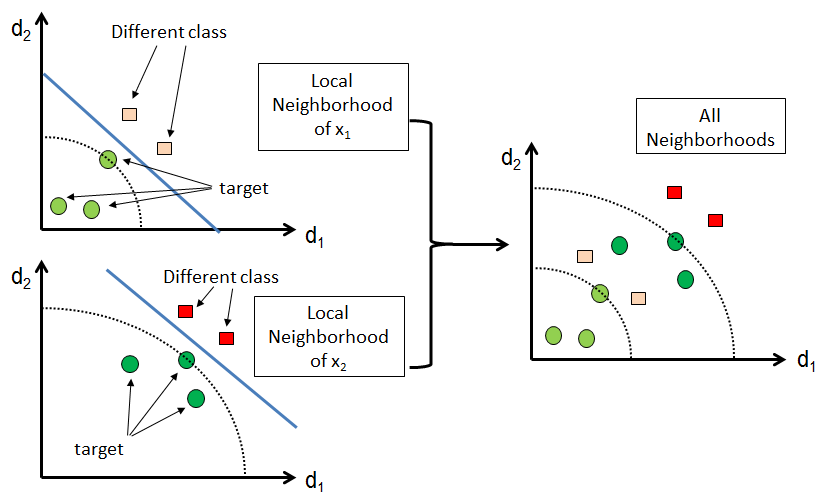
\includegraphics[width=0.8\linewidth]{images/Neighborhood_scaling_problem}
%	\caption{Geometric representation of the neighborhood of $k=3$ for two time series $\textbf{x}_1$ and $\textbf{x}_2$ (left). For each neighborhood, time series of different class are represented by a square and the margin by a blue line. Taking each neighborhood separately, the problem is linearly separable ({\sc lp}/{\sc qp} formulation). By combining the two neighborhoods ({\sc svm} formulation), the problem is no more linearly separable and in this example, the time series of different class of $\textbf{x}_1$ (orange square) are "artificial imposters" of $\textbf{x}_2$. }
%	\label{fig:Neighborhood_scaling_problem}
%\end{figure}


\noindent \textbf{Similarities and differences in the objective function} \\
% \noindent \textbf{Equivalence in the objective function} \\
\noindent Mathematically, from Eq. \ref{eq:pi_plus_A}, we write:
%\begin{equation}
\begin{align}
	\sum\limits_{\substack{i \\ l \in Push_i}}p_i^-\xi_{il} 
	& = 
	\sum_{\substack{i \\ l \in Push_i}} \left( \sum_{\substack{j \in Pull_i}} \frac{1}{2}\right) \xi_{il}\\
	& =
	\sum_{\substack{i \\ j \in Pull_i \\ l \in Push_i}} \frac{\xi_{il}}{2} \label{eq:pi_plus2}
\end{align}
%\end{equation}

\noindent And from Eq. \ref{eq:pi_moins_A}, we write:
\begin{align}
	\sum\limits_{\substack{i \\ j \in Pull_i}}p_i^+\xi_{ij} 
	& =
	\sum_{\substack{i \\ j \in Pull_i}} \left( \sum_{l \in Push_i} \frac{1}{2} \right) \xi_{ij} \\
	& =
	\sum_{\substack{i \\ j \in Pull_i \\ l \in Push_i}} \frac{\xi_{ij}}{2} \label{eq:pi_moins2}
\end{align}

\noindent By replacing Eqs. \ref{eq:pi_plus_A} and \ref{eq:pi_moins_A} back into Eq. \ref{eq:SVMSofMarginProblem1_A}, the objective function becomes:
%\begin{equation}
\begin{align}
	&\displaystyle \argmin_{\textbf{w},\xi} \left\lbrace 
	\frac{1}{2}\textbf{w}^T \textbf{w}
	+ C\sum_{\substack{i \\ j \in Pull_i \\ l \in Push_i}}\frac{\xi_{ij}}{2} 
	+ C\sum_{\substack{i \\ j \in Pull_i \\ l \in Push_i}}\frac{\xi_{il}}{2} \right\rbrace \\
	&\displaystyle \argmin_{\textbf{w},\xi} \left\lbrace 
	\frac{1}{2}\textbf{w}^T \textbf{w}
	+ C\sum_{\substack{i \\ j \in Pull_i \\ l \in Push_i}}\frac{\xi_{ij}+\xi_{il}}{2} 
	+ C\sum_{\substack{i \\ j \in Pull_i \\ k \\l \in Push_k}}\frac{\xi_{ij}+\xi_{kl}}{2} \right\rbrace 
	\\
	&\displaystyle \argmin_{\textbf{w},\xi} \left\lbrace 
	\underbrace{ 
		\vphantom{ \sum\limits_{\substack{i \\ j \in Pull_i \\ k \\l \in Push_k}} }
		\frac{1}{2}\textbf{w}^T \textbf{w}
	}_{Regularization}
	+  C \underbrace{ \left( 
		\sum_{\substack{i \\ j \in Pull_i \\ l \in Push_i}}
		\xi_{ijl} 
	+ \sum_{\substack{i \\ j \in Pull_i \\ k \\l \in Push_k}}
		\xi_{ijkl} 	\right) 
	}_{Loss} \right\rbrace 
	\label{eq:svm2}
\end{align}	
%\end{equation} 
%\noindent The loss-function part of the {\sc svm} problem is similar to the one in Eq.~\ref{eq:MMLPrimalL2}. We can therefore use such {\sc svm}s with kernels to find non-linear forms for the metric $D$:
%
%\begin{align}
%D(\textbf{x}_{i'},\textbf{x}_{j'}) &= \frac{1}{2} 
%\left( \sum\limits_{ij} \alpha_{ij} 	
%y_{ij} 
%K
%\left( 
%\textbf{x}_{ij}
%,	
%\textbf{x}_{i'j'}
%\right) 
%+ b \right) 
%\label{Eq:nonlinearDSVM}		
%\end{align}

%In this section, we investigate the similarities and the differences between the {\sc lp}/{\sc qp} and {\sc svm} formulations. \\
\noindent the {\sc svm} formulation (Eq. \ref{eq:SVMSofMarginProblem1_A}) and the {\sc m$^2$tml} formalization (Eq.~\ref{eq:quadratic_A}) share a same loss term involving the slack variables $\xi_{ijl}$ (push cost). However, the {\sc svm} formulation includes additionnal slack variables $\xi_{ijkl}$ due to the additional set of constraints. \\
\noindent In the {\sc svm} formulation (Eq. \ref{eq:SVMSofMarginProblem1_A}), the regularization part tends to minimize the norm of $\textbf{w}$ whereas in {\sc m$^2$tml} (Eq.~\ref{eq:quadratic_A}), it tends to minimize the norm of $\textbf{w}$ after a linear transformation through the matrix $\textbf{M}$ (pull cost). 
% Even if the loss part (push cost) is the same for both objective functions, the regularization part (pull cost) is different. In the {\sc svm} formulation (Eq. \ref{eq:SVMSofMarginProblem1_A}), the regularization part tends to minimize the norm of $\textbf{w}$ whereas in {\sc m$^2$tml} (Eq.~\ref{eq:quadratic_A}), it tends to minimize the norm of $\textbf{w}$ after a linear transformation through $\textbf{X}_{tar}$. This transformation can be interpreted as a Mahalanobis norm in the dissimilarity space with $\textbf{M}=\textbf{X}_{tar}\textbf{X}_{tar}^T$. Nevertheless, both have the same objective: improve the conditioning of the problem by enforcing solutions with small norms. In practice, even with these differences, the {\sc svm} provides suitable solutions for our time series metric learning problem. \\
%($\textbf{X}_{tar}.\textbf{X}_{tar}^T$ can be seen as a specific choice of Tikhonov matrix). 


%%% Local Variables: 
%%% mode: latex
%%% TeX-master: "../roque-phdthesis"
%%% End: 
